\documentclass{article}
\usepackage{graphicx} %package to manage images
\graphicspath{ {./figures/} }
\usepackage{hyperref}
\usepackage{caption}
\usepackage[font=scriptsize]{subcaption}
\captionsetup[figure]{labelsep=none}
\captionsetup[table]{labelsep=none}
\usepackage{bbm}
\usepackage{amsmath}
\usepackage{import}
\usepackage{array}
\usepackage{booktabs}
\usepackage{afterpage}
\usepackage{floatrow}
\usepackage{pdflscape}
\usepackage{soul}
\usepackage{float}
\usepackage{adjustbox}
\usepackage{longtable}


\title{maternal nutrition by social group}

\date{April 2025}

\begin{document}

\maketitle


\section{outcome: BMI}
\begin{figure}[H]
    \centering
    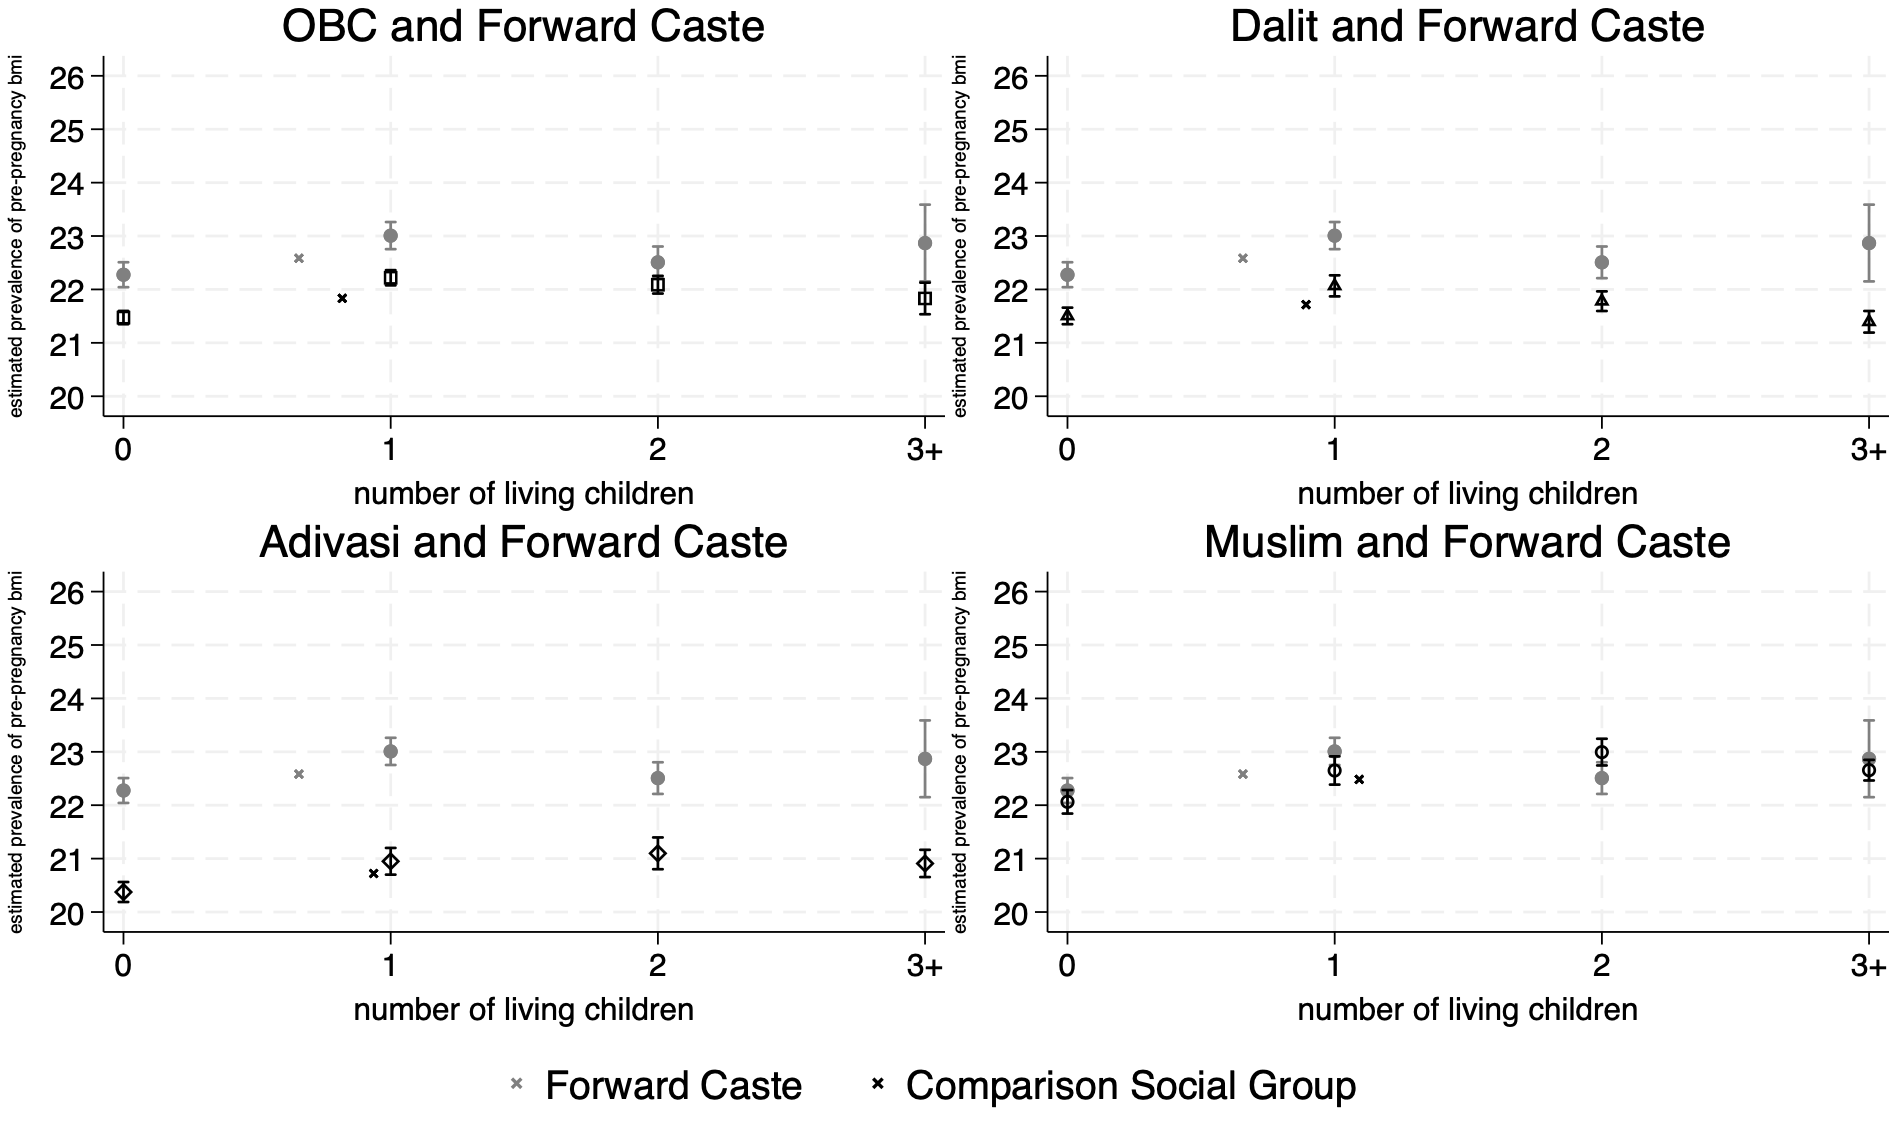
\includegraphics[width=\textwidth]{figures/maternal nutrition by social group/prepreg_bmi_combined.png}
\end{figure}

\section{outcome: underweight}
\begin{figure}[H]
    \centering
    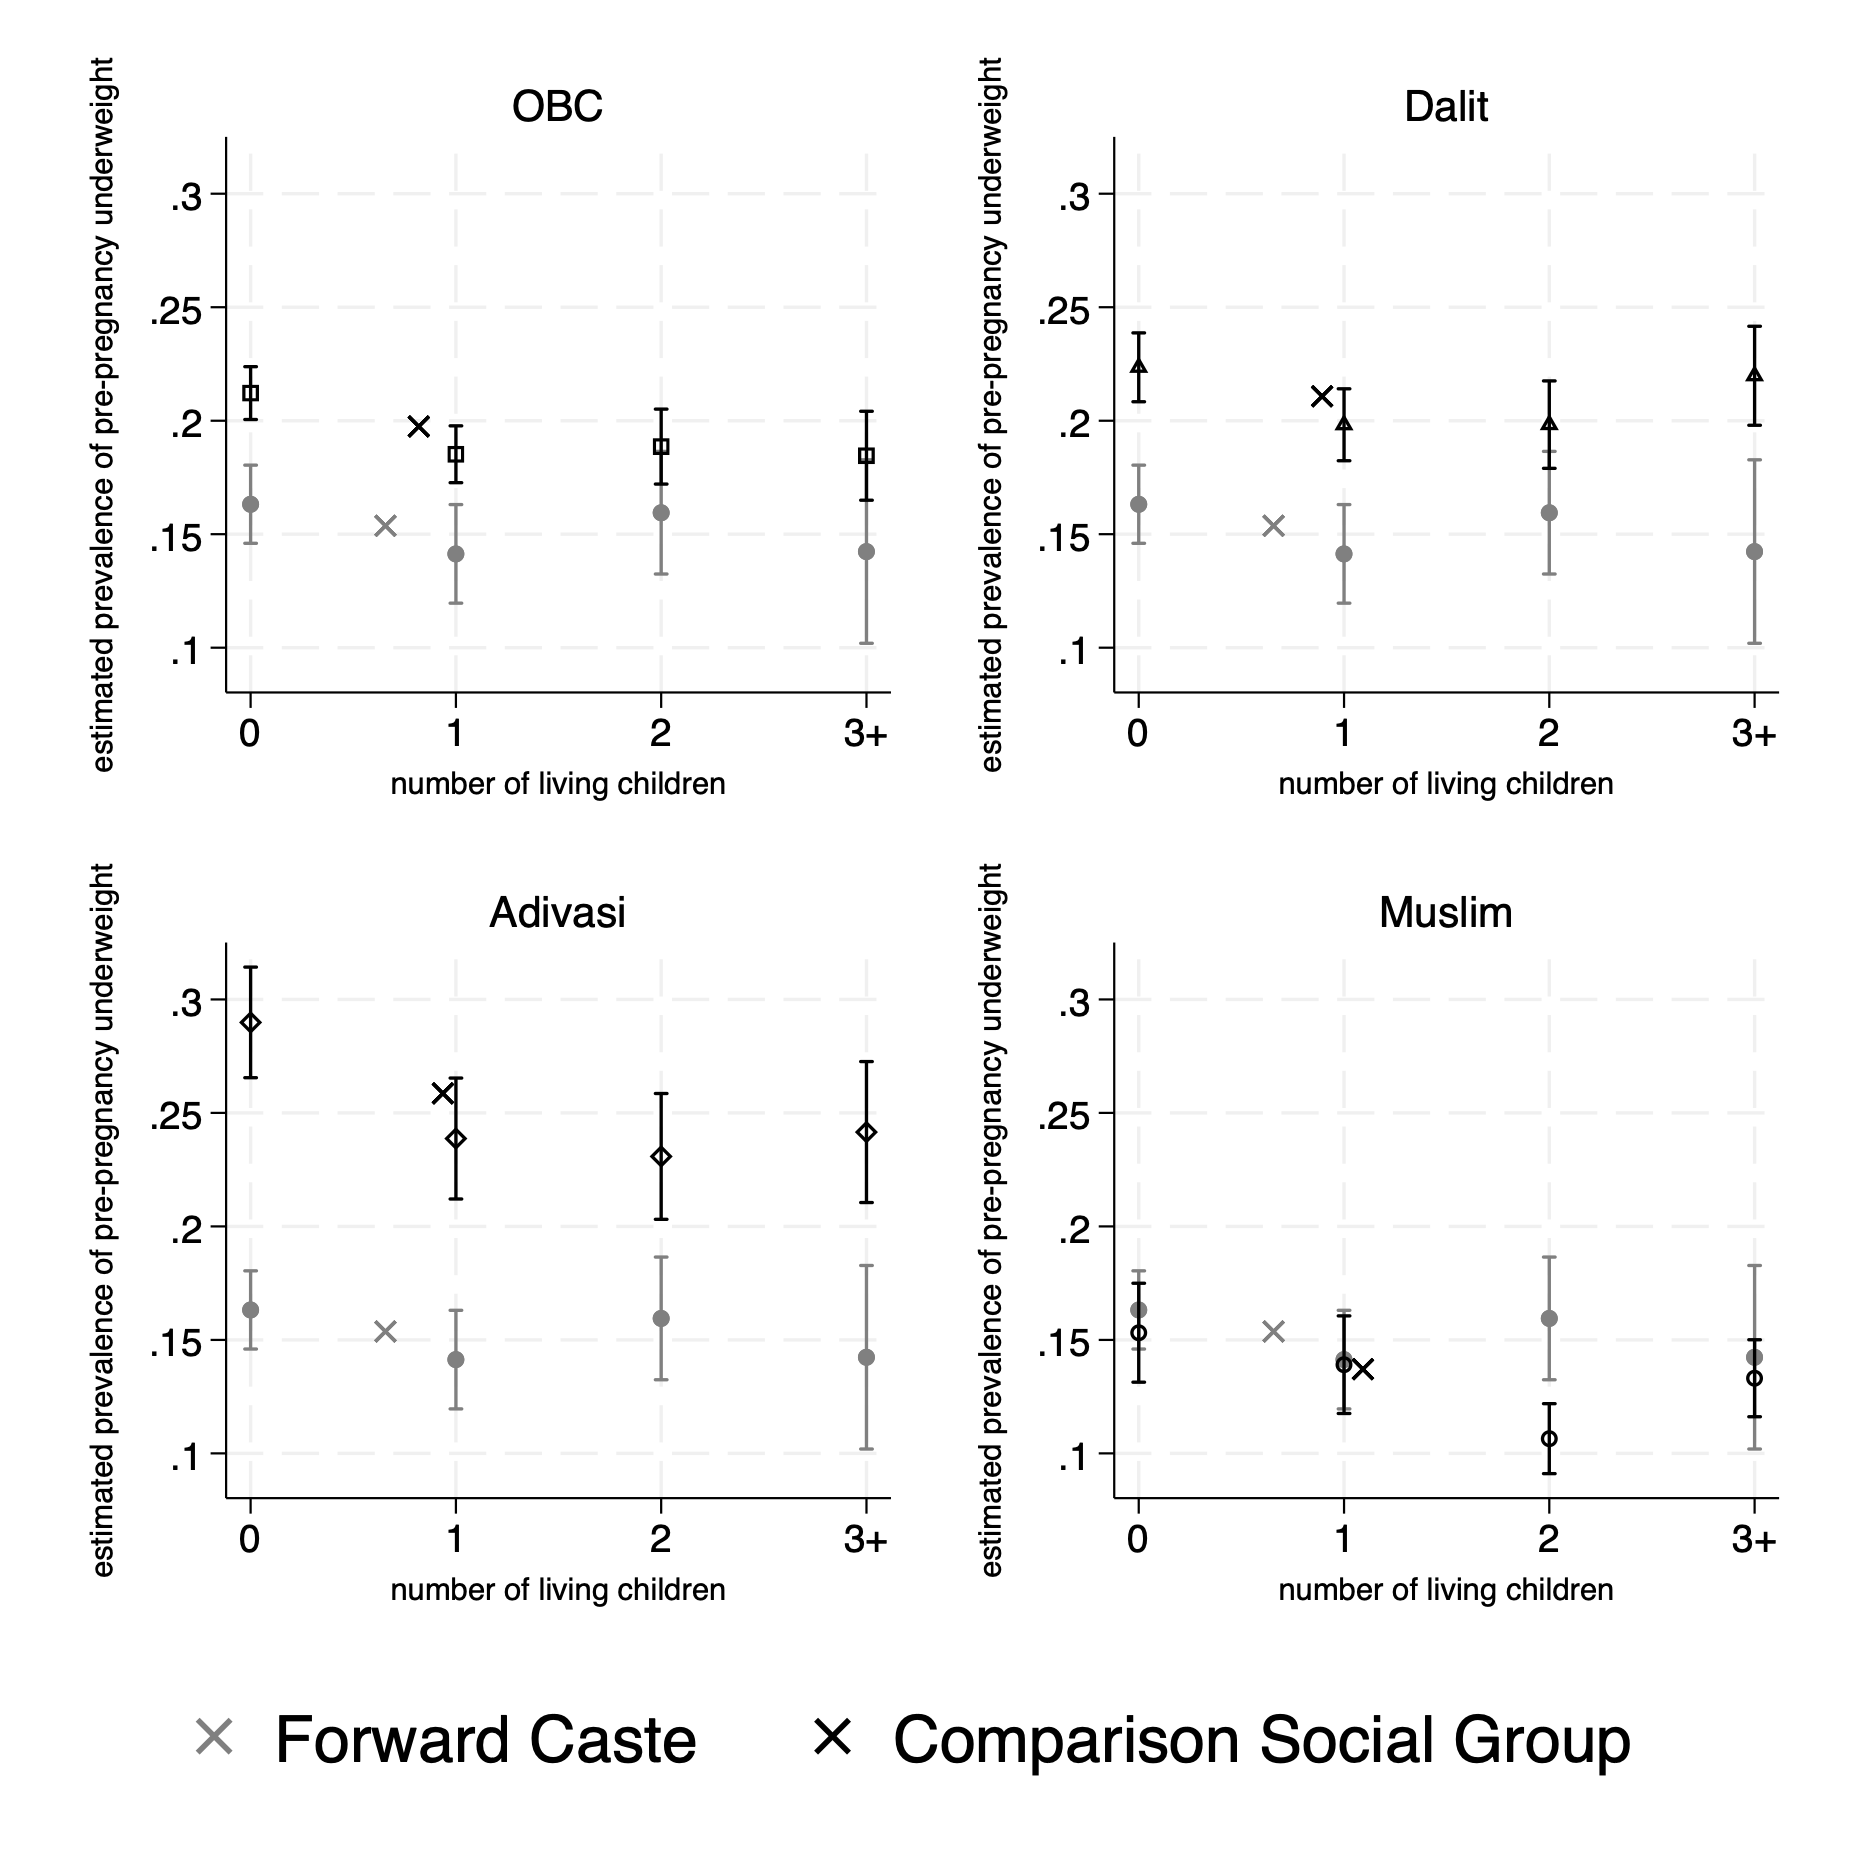
\includegraphics[width=\textwidth]{figures/maternal nutrition by social group/prepreg_underweight_combined.png}
\end{figure}

\section{stacked bar graph}
\begin{figure}[H]
    \centering
    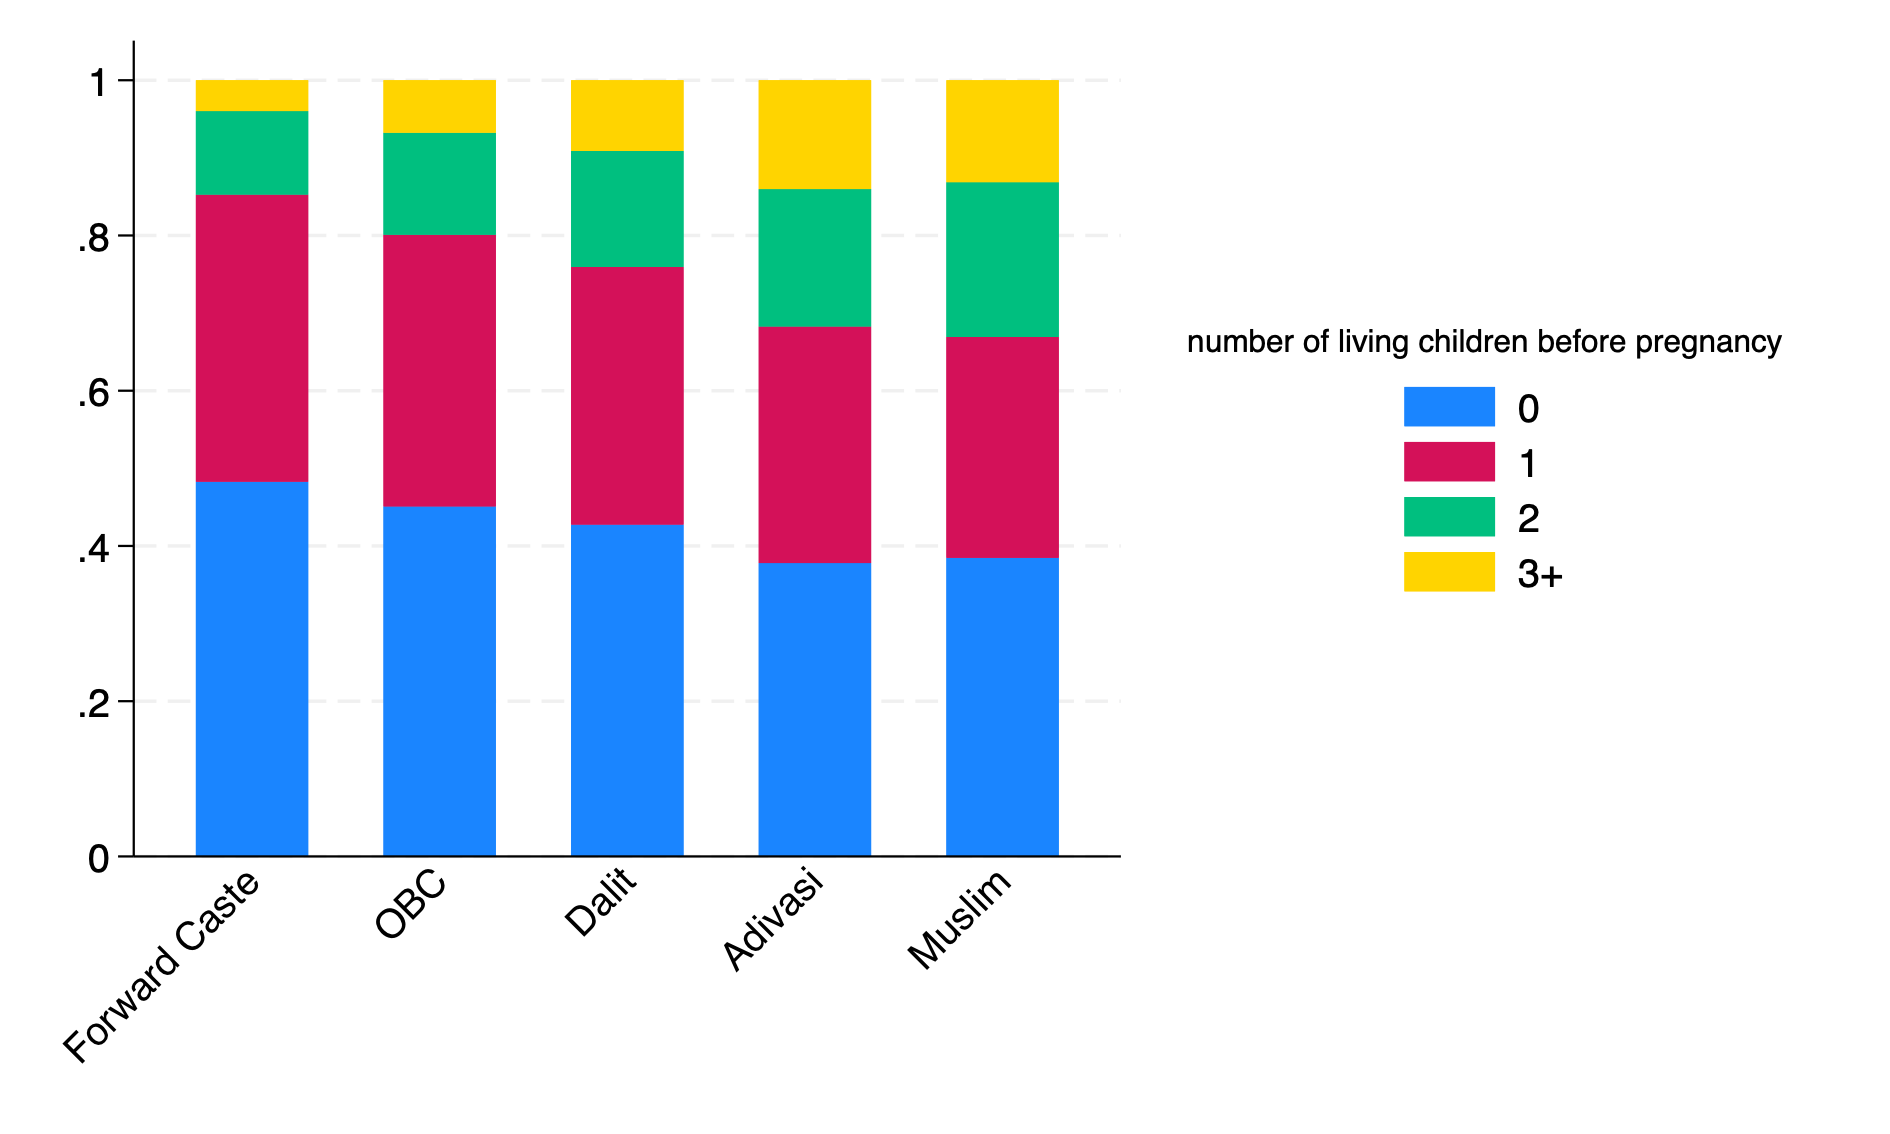
\includegraphics[width=\textwidth]{figures/maternal nutrition by social group/stackedbar_parity_socialgroup.png}
\end{figure}




\end{document}
